\section{Development of organisms and continuity of life}
\subsection{Nuclear division}

Chromosomes, present in the nucleus and that on which genetic information is stored, are structures
made of DNA.

A haploid nucleus is that which contains a single set of chromosomes, a diploid one contains two
sets. For humans, a diploid nucleus contains 46 chromosomes and a haploid nucleus contains 23.

Mitosis is a form of nuclear division which gives rise to genetically identical cells in which
the chromosome number of daughter cells is maintained and equal to mother cell and sibling cells.

\begin{center}
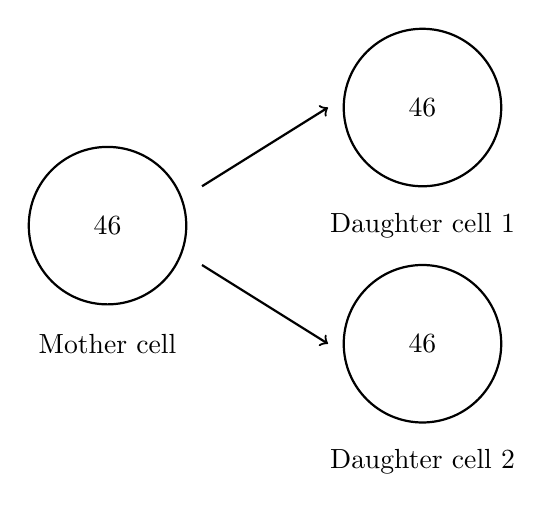
\begin{tikzpicture}
% Mother cell
\draw[thick] (0,0) circle(1); % Mother cell
\node at (0,0) {46}; % Chromosome count
\node at (0,-1.5) {Mother cell};

% Arrows for division
\draw[->,thick] (1.2,0.5) -- (2.8,1.5);
\draw[->,thick] (1.2,-0.5) -- (2.8,-1.5);

% First daughter cell
\draw[thick] (4,1.5) circle(1); % Daughter cell 1
\node at (4,1.5) {46}; % Chromosome count
\node at (4,0) {Daughter cell 1};

% Second daughter cell
\draw[thick] (4,-1.5) circle(1); % Daughter cell 2
\node at (4,-1.5) {46}; % Chromosome count
\node at (4,-3) {Daughter cell 2};
\end{tikzpicture}
\end{center}
The above diagram shows a mother cell dividing, by mitosis, into two daughter cells with the same
number of chromosomes. The cells produced are genetically identical. An organism grows or repairs
parts of its body by mitosis. In other words, mitosis plays the role of growing the body and 
replacing deprecated cells. Mitosis is also used in asexual reproduction, for example, when
potatoes grow new plants from tubers, the new plants form by mitosis, meaning they are all 
genetically identical.

Stem cells are unspecialised cells that divide by mitosis to produce daughter cells that can become
specialised for specific functions. In the bone marrow, there are stem cells from whose mitosis
divisions blood cells form. Stem cells in the brain divide to form new neurones.

Meiosis is the type of cell division involved in the production of gametes. Meiosis division is
a reduction division in which chromosome number is halved from diploid to haploid, resulting in
genetically different cells.

\begin{center}
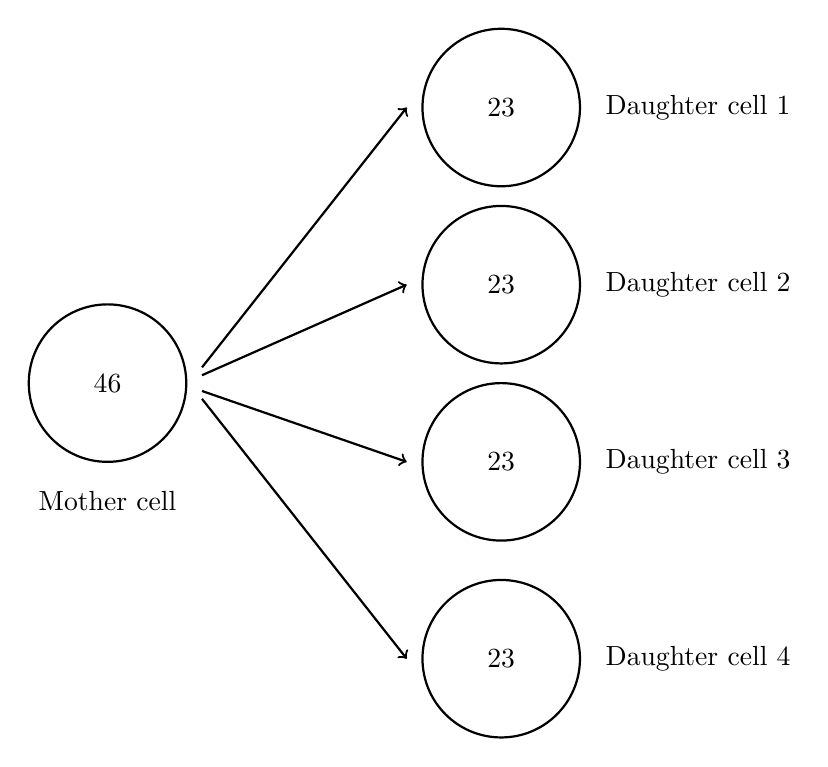
\begin{tikzpicture}
% Mother cell
\draw[thick] (0,0) circle(1); % Mother cell
\node at (0,0) {46}; % Chromosome count in mother cell
\node at (0,-1.5) {Mother cell};

% Arrows for division
\draw[->,thick] (1.2,0.2) -- (3.8,3.5);
\draw[->,thick] (1.2,0.1) -- (3.8,1.25);
\draw[->,thick] (1.2,-0.1) -- (3.8,-1);
\draw[->,thick] (1.2,-0.2) -- (3.8,-3.5);

% First daughter cell
\draw[thick] (5,3.5) circle(1); % Daughter cell 1
\node at (5,3.5) {23}; % Chromosome count
\node at (7.5,3.5) {Daughter cell 1};

% Second daughter cell
\draw[thick] (5,1.25) circle(1); % Daughter cell 2
\node at (5,1.25) {23}; % Chromosome count
\node at (7.5,1.25) {Daughter cell 2};

% Third daughter cell
\draw[thick] (5,-1) circle(1); % Daughter cell 3
\node at (5,-1) {23}; % Chromosome count
\node at (7.5,-1) {Daughter cell 3};

% Fourth daughter cell
\draw[thick] (5,-3.5) circle(1); % Daughter cell 4
\node at (5,-3.5) {23}; % Chromosome count
\node at (7.5,-3.5) {Daughter cell 4};

\end{tikzpicture}
\end{center}
As shown above, meiosis gives rise to four genetically different daughter cells. Which daughter 
cell gets which combination of the haploid chromosomes is random, and hence the genetic 
characteristics of the daughter cells of this division is random.

Cancers are a result of defective cells dividing uncontrollably.

\subsection{Asexual and sexual reproduction}

Asexual reproduction is a procuss by which genetically identical offspring are produced by a single
parent. Unicellular organisms usually undergo this form of reproduction, alongside some species
of plants under certain situations. The process is faster as mates need not be found and the
genetic characteristics of the offspring are perfectly predictable. However, asexual reproductions
may reduce the biological diversity of a habitat and genetic disorders may arise in offspring.
Asexual reproduction is advantageous for a species newly colonising a new environment, to which
it is well suited. It can then reproduce quickly by mitosis and reap the benefits of the area.

Sexual reproduction is a proces involving the fusion of haploid nuclei, a process known as 
fertilisation, to form a diploid zygote and the production of genetically different offspring. 
These haploid nuclei, or rather, the cells containing these haploid nuclei are called gametes. The
zygote that results from their fusion is haploid. Sexual reproduction gives rise to genetic
disparity amongst parent and child, giving rise to biodiversity. Yet it is slow for the same
reasons meiosis is fast. There is also less chance of genetic diseases arising. Sexual reproduction
allows an organism to adapt to its surroundings, and is useful when new areas are being colonised.

\subsection{Sexual reproduction in plants}

A flowering plant produces structures called flowers. They consist of the sepals, which are leaf
like structures that surround the flower by formning a ring around the flower petals. The
petals of a flower are coloured structures that attract insects or birds to it. The stamens of a
flower are the male parts of the flower, which consist of a filament and anther, the stalk part
and the pollen producing and containing part of the flower respectively. Pollen grains are 
strructures of a flower containing the male gametes of the flower. The carpel is the female part
of the flower, consisting of the ovary which holds the ovules, which are small structures 
containing the female gametes. The style is the part of the carpel connecting the stigma to the
ovary. The stigma is the part of the flower that recieves the pollen.

Pollination is the process by which pollen is carried from the anther of a flower to the stigma
of a flower of the same species. It is done by two means, by insects or by wind, and plants 
utilising these strategies are adapted accordingly.

In plants which are pollinated by insects, the filament is relatively short resulting in the
anthers being inside the flower. They have large, attractive petals to attract insects and to act
as landing pads for them. Such flowers may have nectar to attract the insects into the flower. 
Pollen brushes onto the insects body from the anthers as it tries to get the nectar. When the
insect flies to another flower looking for nectar, it carries the pollen to that flower, where
the flower becomes pollinated. The pollen grains in such plants tend to be rough so as to stick
to the pollinating insects. Such plants may be strongly scented. Insect pollinated flowers produce
less quantities of pollen than wind pollinated flowers as it is a more surefire method of 
pollination.

In plants pollinated by the wind, pollen have smooth shapes with large surface area to be carried
easily by the wind. The filaments are long and the anthers hang out of the flower in such plants,
to maximise the chance of wind carrying the pollen to another flower of the same species. The
stigma of such flowers tend to also be stuck out of the flower, to maximise chance of catching
the floating pollen. They tend to have shapes that maximise their surface area for the same reason.
Such flowers lack particularly attractive petals and nectar as there is no need to attract any
insect. Wild pollinated flowers lack any scent at all. Such flowers produce huge quantities of
pollen to maximise chance of pollination as most will not reach a stigma. Pollen from such plants
tend to be quite lightweight to be carried easily by the wind.

Pollination can occur between the male and female parts of the same flower, or the different
flowers of the same plant. This is known as self pollination. This results in loss of biodiversity
as produced zygotes form a similar genetic makeup. Minimal genetic variation will result from such
pollination. Genetic diseases may arise.

Pollination occuring between male and female parts of different plants altogether is called cross
pollination. This gives rise to genetic variation, allowing the plant to adapt to changes in
environment and increases biodiversity. There is no chance of genetic diseases arising in such a
form of pollination.

After pollination, enzymes in the pollen digest through the stigma of the flower to make a path
for the male nucleus (gamete) to merge with the female gamete, which is in the ovule, in the ovary.
The pollen tube grows into the ovule through a small tube called the micropyle, after which the
male gamete travels down the pollen tube and into the ovule where it fuses with the female gamete.
This is fertilisation.

Subsequent to fertilisation, most of the flower is redundant. Petals, sepals and stamens all dry,
shrink and wither before falling off. The zygote containing ovule divides by mitosis to form an
embryo plant, now called a seed. The ovary develops into a fruit. 

The thick, hard, outermost layer of the seed is called the seed coat or testa. It prevents entry of
water into the seed. The seed itself is kept dehydrated to slow down metabolic reactions in it
significantly to keep it dormant. The embryo in the seed is attached to two leave like structures
called cotyledons, which are swollen with stored food. Plants that contain two of such leaves are
called dicotyledonous and those with one of them are called monocotyledonous. Cotyledons contain
stored food, mostly in the form of starch. The plumule is the part of the seed that will develop
into the shoot and the radicle is that which will develop into the root.

Dispersal of seeds by animals is a means of colonising new areas and reducing competition around
the home area. Such seeds tend to have sweet fruits so as to be ingested by animals, and as the
seed emerges unscathed through the animals alimentary canal, it will be left in a condition
to be germinated, the process through which the seed changes to a plant. Seeds may also be wind
dispersed, in which case they are light and have a large surface area so as to be able to be carried
effectively by the wind to a region suitable to germinate.

When the seed is in a situation with the following: water, oxygen and a suitable temperature, it
may germinate. Enzymes in the seed work to digest the storeed food into soluble forms in the seed,
which is then carried to the growing regions of the embryo. However, germinated seeds may not 
mature, as some seedlings compete for light due to overcrowding, unsuitable temperature also causes
death of sedlings and lack of ions or minerals may stunt growth. Starch is broken down to glucose
to be used in respiration during germination, amino acids are used to build up proteins using this
energy to make the cytoplasm and cell membranes of the new cells. Lipids are synthesised for the
same purpose.

\subsection{Sexual reproduction in humans}

The male reproductive system in humans consists of the testes, glands which produce sperm; the 
scrotum, a sack like structure holding these testes; sperm ducts are tubes which
carry sperm from the testes to the penis; where the sperm duct connects to the penis, a gland
called the prostate gland produces semen and mixes it with the sperm.

In females, the reproductive system consists of the ovaries, where the egg cells are made; leading
out of the ovaries are oviducts which lead eggs into the womb or uterus, a structure consisting
of very thick, extremely stretchy walls which do so when as this is where the foetus is when the
woman is pregnant. The narrow opening to the uteris is called the cervix, after which lies the
vagina which leads to outside the body.

A sperm cell is the male human gamete. It consists of a flagellum, a tail like structure which
enables the cell to be mobile. The middle piece of the cell contains mitochondria to release
energy for swimming. The head of the sperm cell consists of an acrosome, which is a vesicle 
containing enzymes to digest through the jelly coat of an egg cell. The head also contains the
male haploid nucleus, alongside more mitochondria to release energy for the cell's swimming 
movement. Sperm cells are produced in the testes and they are produced and released millions
at a time.

An egg cell is significantly larger than a sperm cell, yet a sperm cell is longer than an egg
cell due to its flagellum; it consists of a jelly coat surround the
cell surface membrane. Inside the cell the cytoplasm contains ``yolk", which is an energy store.
The nucleus of the egg cell is haploid. The jelly coat of an egg cell changes when a sperm has
fertilised the egg cell, so as to not allow any other sperm to fertilise that egg cell. Egg cells
are not produced in high numbers, and a female has a limited store of them, around middle age, a
female will no longer have any egg cells.

Testosterone is the male sexual hormone. During their early teenage years, boys' testes start
producing this hormone causing them to develop secondary sexual characteristics such as body and
facial hair and to start producing sperm. Oestrogen is that in girls, for whom secondary sexual
characteristics consist of breasts, monthly menstruation cycles and also body hair.

In women, the menstrual cycle is a monthly hormonal cycle consisting of the release of an egg
cell and changing of the uterine lining. This cycle is regulated by four hormones: the follicle
stimulating hormone (FSH), luteinising hormone (LH), oestrogen and progesterone, namely. The latter
two are released by the ovaries whereas the remaining are released by the pituitary gland in the
brain.

At the
beginning of the cycle (usually the start of a month), FSH levels are high, stimulating the 
development of an egg cell in an egg follicle. This developing follicle secretes oestrogen in
increasing amounts, which stimulates repair of the uterus lining, makin git thicker and better
supplied with blood. When the follicle is fully developed, a surge in LH causes ovulation, in which
the egg cell breaks free from the follicle, the remaining follicle is called the corpus luteum. 
This corpus luteum secretes progesterone which maintains the state of the uterine lining. 
Progesterone inhibits production of FSH and LH, so no new follicles are stimulated and no more
eggs are ovulated. If the egg is not fertilised, the uterine lining breaks down as a result of
progesterone secretion stopping. FSH and LH start increasing and the cycle repeats.

The egg cell is fertilised by a sperm cell in the oviduct. After fertilisation, the zygote moves
down the oviduct while dividing, it has now become an embryo after having turned into a ball of 
cells. The uterus has a thick, spongy lining, into which the embryo sinks, called implantation.

As the embryo grows, a placenta also grows which connects the embryo to the wall of the uterus.
It is a soft, dark red structure with projections similar to the villi in the small intestine. 
Here nutrients and waste substances are exchanged between the mother's blood and the foetus's blood.
These two blood mixtures never mix, only flow very close to each other. As the foetus grows, an
umbilical cord also forms through blood vessels in which foetal blood goes to and from the placenta.

Some pathogens, such as HIV can pass the placenta. Carbon monoxide and alcohol are toxins which can
also cross the placenta. This will negatively affect the foetus's growth.
